\documentclass[a4paper,10pt]{article}
\usepackage[utf8]{inputenc}
\usepackage{cite}
\usepackage[top=2.5cm,bottom=2.5cm,left=2.5cm,right=2.5cm]{geometry}
\usepackage[portuguese]{babel}
\usepackage{natbib}
\usepackage{graphicx}
\usepackage{url}



\title{Comércio Eletrônico}
\author{Mader Gabriel de Souza Barbosa}
\date{April, 2022}

\begin{document}

\maketitle

\begin{figure}[h!]
\centering
    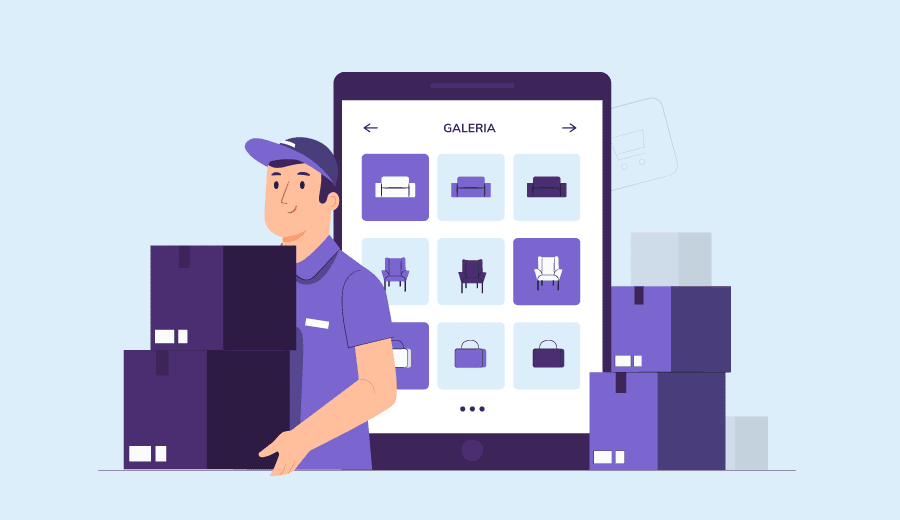
\includegraphics[width=80mm]{ecommerce.png}
    \caption{Ilustração sobre \textit{E-commmerce}. \cite{img:graph}}
    \label{fig:graph1}
\end{figure}

\section{Introdução}
\paragraph 
O comércio eletrônico(ou /textit{E-commerce}) se refere a todas as transações online, sendo inclusa uma ampla gama de atividades online e ferramentas. Se tornando uma das principais alternativas para aumento de ganhos em negócios\cite{img:graph}. Tendo em vista seu grande impacto global, existe uma cadeira eletiva no Centro de Informática(UFPE)  que possui 75 horas de carga horária e visa o estudo e ensino do comércio eletrônico e suas nuances, que é a cadeira IF792.


\section{Relevância}
\paragraph
Pela facilidade de fazer uma compra no conforto de sua casa e pelo fato de ter ocorrido um lockdown devido à pandemia de COVID=19 no mundo todo, o comércio eletrônico se tornou algo indispensável na vida dos cidadãos. No Brasil, mais de 7 milhões de brasileiros fizeram uma compra online pela primeira vez no 1º semestre de 2020 \cite{fonte:xxx} o que representa uma relação direta com o auge do isolamento social na maioria das cidade brasileiras. Devido ao grande aumento de consumidores, ficou cada vez mais importante a presença do comércio eletrônico na sociedade, tanto como um complemento ao modelo de negócio convencional, tanto comoforma de impulsionar as vendas e alcançar diferentes públicos. Pois, além de sua importância com vendas diretas, o \textit{E-commerce} é uma ferramenta de marketing que auxilia na divulgação de produtos, marcas e serviços.\cite{fonte:xxb} Tendo em vista isso, a necessidade de se ter uma cadeira para estudar e se especializar nessa área se torna indispensável para o Centro de Informática(UFPE).


\section{Relações com outras disciplinas}
\paragraph
Apesar de não necessitar de pré requisito para que a matricula seja feita, a disciplina de comércio eletrônico(IF792), por ser uma disciplina eletiva, irá utilizar alguns conceitos de computação que uma pessoa que não tem conhecimento prévio de matérias dadas nos primeiros períodos do Cin, provavelmente não conseguirá prosperar nesta cadeira, mesmo que não estejam listados de forma obrigatória. Além disso, por ser uma cadeira que é voltada para a área de negócios e empreendedorismo, ela possui relações com outras cadeiras eletivas como gestão de negócios(IF783), negócios online (IF782) e economia para empreendedor (IF780) por serem ligadas à negócios.



\bibliographystyle{plain}
\bibliography{mgsb.bib}

\end{document}
